% ============================================================================
% REQUIRED PACKAGES & CONFIGURATIONS FOR COMPILING THIS EXPERIMENT:
%  ----------------------------------------------------------------------------
% \usepackage{circuitikz}      % For drawing op-amp circuit schematics
% \usepackage{pgfplots}        % For professional signal waveforms
% \pgfplotsset{compat=1.18}    % Ensures modern rendering engine defaults
% \usepackage{booktabs}        % For publication-grade tables
% \usepackage{amsmath}         % For advanced mathematical formulas
% \usepackage{siunitx}         % For standard scientific units (\SI, \kilo\omega, etc.)
%
% Done by Gemini.
% ============================================================================

\chapter{Adder and Subtractor Using Op-amps}

\section{Aim}
To design, assemble, and experimentally verify the performance of Operational Amplifier (Op-Amp) mathematical circuits using IC 741. The specific objectives are:
\begin{enumerate}
	\item To implement an Inverting Summing Amplifier (Adder) and verify that $V_{out} = -(V_1 + V_2)$.
	\item To implement a Difference Amplifier (Subtractor) and verify that $V_{out} = V_2 - V_1$.
	\item To observe and record the input and output waveforms for both DC and AC input signals.
\end{enumerate}

\section{Pre-Lab Assignment}
\begin{enumerate}
	\item Review the virtual-short and zero-input-current assumptions of the ideal op-amp and their application to circuits with multiple input signals.
	\item For a summing amplifier with two/three inputs and a target output relationship assigned to your batch (e.g., $v_{out} = -(v_1 + v_2)$), design the required resistor values.
	\item For a difference amplifier with a target gain assigned to your batch, design the required resistor values, ensuring the condition for common-mode rejection (Equation~\eqref{eq:cmrr_condition}) is satisfied.
	\item Simulate both designed circuits in LTspice with appropriate DC and/or sinusoidal sources at each input, and verify the expected output algebraically combines the inputs as designed.
\end{enumerate}

\section{Components and Equipment Required}
The components and test instruments required for this experiment are listed in Table \ref{tab:components_opamp2}.

\begin{table}[h!]
	\centering
	\begin{tabular}{@{}cll@{}}
		\toprule
		S.No. & Component/Equipment & Specification \\
		\midrule
		1  & Operational Amplifier IC & $\mu$A741 (or equivalent), 1 no. \\
		2  & Resistors & $R_1, R_2, R_3, R_f$ as per design \\
		3  & Dual Regulated DC Power Supply & $\pm 15\,\text{V}$ \\
		4  & Function Generator(s) & Sine wave, 1\,Hz -- 1\,MHz (2 nos., if available) \\
		5  & Additional DC Power Supply & 0--5\,V (for DC input levels) \\
		6  & Digital Storage Oscilloscope & 2-channel, 20--50\,MHz bandwidth \\
		7  & Digital Multimeter & For DC voltage measurements \\
		8  & Breadboard and connecting wires & -- \\
		\bottomrule
	\end{tabular}
	\caption{Components and equipment list.}
	\label{tab:components_opamp2}
\end{table}

\section{Theory}
Operational amplifiers can perform linear mathematical operations directly on analog voltage signals. Negative feedback forces the differential input voltage to near zero, simplifying circuit analysis through the virtual short/ground approximation.

\subsection{Inverting Summing Amplifier (Adder)}
In an inverting summing configuration, multiple input voltages are connected through individual resistors to the inverting input terminal (pin 2) of the op-amp. The non-inverting terminal (pin 3) is connected to ground through an offset-minimizing resistor $R_{comp}$.

Because the inverting node is maintained at virtual ground ($0\text{ V}$), Kirchhoff's Current Law (KCL) at the summing junction gives:
\begin{equation}
	I_1 + I_2 = I_f \implies \frac{V_1 - 0}{R_1} + \frac{V_2 - 0}{R_2} = \frac{0 - V_{out}}{R_f}
\end{equation}
Rearranging for $V_{out}$:
\begin{equation}
	V_{out} = - \left( \frac{R_f}{R_1} V_1 + \frac{R_f}{R_2} V_2 \right)
\end{equation}
When all resistors are equal ($R_1 = R_2 = R_f = R$):
\begin{equation}
	V_{out} = -(V_1 + V_2)
\end{equation}
The negative sign indicates an overall $180^\circ$ inversion of the sum.

\subsection{Difference Amplifier (Subtractor)}
A difference amplifier amplifies the potential difference between two input signals while rejecting any common-mode voltage. $V_1$ is fed to the inverting input via $R_1$, and $V_2$ is fed to the non-inverting input via a voltage divider formed by $R_3$ and $R_4$.

Applying the superposition principle:
\begin{enumerate}
	\item With $V_2 = 0\text{ V}$, the circuit acts as an inverting amplifier: $V_{out1} = -\frac{R_2}{R_1} V_1$.
	\item With $V_1 = 0\text{ V}$, the voltage at the non-inverting pin is $V_+ = V_2 \left(\frac{R_4}{R_3 + R_4}\right)$. The circuit acts as a non-inverting amplifier:
	\begin{equation}
		V_{out2} = V_+ \left( 1 + \frac{R_2}{R_1} \right) = V_2 \left( \frac{R_4}{R_3 + R_4} \right) \left( \frac{R_1 + R_2}{R_1} \right)
	\end{equation}
\end{enumerate}
Combining both contributions yields the net output:
\begin{equation}
	V_{out} = V_{out1} + V_{out2} = V_2 \left( \frac{R_4}{R_3 + R_4} \right) \left( \frac{R_1 + R_2}{R_1} \right) - \frac{R_2}{R_1} V_1
\end{equation}
If $R_1 = R_3$ and $R_2 = R_4$:
\begin{equation}
	V_{out} = \frac{R_2}{R_1} (V_2 - V_1)
\end{equation}
For unity differential gain ($R_1 = R_2 = R_3 = R_4 = R$):
\begin{equation}
	V_{out} = V_2 - V_1
\end{equation}

\section{Circuit Diagram}
The schematics for the Inverting Adder and Subtractor are shown in Figures \ref{fig:adder_circuit} and \ref{fig:subtractor_circuit}.

\begin{figure}[h!]
	\centering
	\begin{circuitikz}[scale=0.9,line width=0.8pt, transform shape]
		% Op-amp
		\draw (0,0) node[op amp] (opamp) {LM 741};
		
		% Summing Junction Node
		\draw (-2, 0.5) node[circle, fill, inner sep=1.5pt] {} -- (opamp.-);
		
		% Input 1 Path
		\draw (-2, 0.5) -- (-2, 1.5) to[R, l_=$R_1\ (\SI{10}{\kilo\Omega})$] (-5.5, 1.5) to[sV, l_=$V_1$] (-5.5, 0) node[ground] {};
		
		% Input 2 Path
		\draw (-2, 0.5) -- (-2, -0.5) to[R, l_=$R_2\ (\SI{10}{\kilo\Omega})$] (-4.5, -0.5) to[sV, l_=$V_2$] (-4.5, -2) node[ground] {};
		
		% Non-inverting Compensation
		\draw (opamp.+) to[R, l_=$\SI{3.3}{\kilo\Omega}$] (-1.2, -2) node[ground] {};
		%\draw (opamp.+) to[R, l_=$R_{comp}$] (-1.2, -2) node[ground] {};
		
		% Feedback Loop
		\draw (-2, 0.5) -- (-2, 2.7) to[R, l=$R_f\ (\SI{10}{\kilo\Omega})$] (1.5, 2.7) -- (1.5, 0) -- (opamp.out);
		
		% Output
		\draw (opamp.out) -- (2.5, 0) node[right] {$V_{out}$};
		
		% Vertical Power Lines
		\draw (opamp.up) -- ++(0, 0.5) node[above] {$+15\text{ V}$};
		\draw (opamp.down) -- ++(0, -0.5) node[below] {$-15\text{ V}$};
		
		% Connection Dot
		\node[circle, fill, inner sep=1.5pt] at (1.5, 0) {};
		\node[circle, fill, inner sep=1.5pt] at (-2, 1.5) {};
		% Pin numbers attached to terminal anchors
		\node[font=\small, above right] at (opamp.-) {2};   % Inverting Input
		\node[font=\small, above right] at (opamp.+) {3};   % Non-Inverting Input
		\node[font=\small, above left]  at (opamp.out) {6}; % Output
		\node[font=\small, above right] at (opamp.up) {7};  % +VCC
		\node[font=\small, below right] at (opamp.down) {4};% -VEE
	\end{circuitikz}
	\caption{Inverting Summing Amplifier (Adder) Circuit Diagram}
	\label{fig:adder_circuit}
\end{figure}

\begin{figure}[h!]
	\centering
	\begin{circuitikz}[scale=0.9, line width=0.8pt, transform shape]
		% Op-amp
		\draw (0,0) node[op amp] (opamp) {LM 741};
		 %(-2, 0.5) -- (-2, 1.5)
		% Inverting Input Path (V1)
		\draw (opamp.-) -- (-2, 0.5) to[R, l_=$R_1\ (\SI{10}{\kilo\Omega})$] (-5.5, 0.5) to[sV, l_=$V_1$] (-5.5, -2) node[ground] {};
		
		% Inverting Feedback Path
		\draw (-1.5, 0.5) -- (-1.5, 2) to[R, l=$R_2\ (\SI{10}{\kilo\Omega})$] (1.5, 2) -- (1.5, 0) -- (opamp.out);
		
		% Non-Inverting Path (V2 + Divider R3, R4)
		\draw (opamp.+) -- (-1.5, -0.5) to[R, l_=$R_3\ (\SI{10}{\kilo\Omega})$] (-4, -0.5) to[sV, l_=$V_2$] (-4, -2) node[ground] {};
		\draw (-1.5, -0.5) to[R, l_=$R_4\ 10\ k\Omega$] (-1.5, -2.2) node[ground] {};
		
		% Output
		\draw (opamp.out) -- (2.5, 0) node[right] {$V_{out}$};
		
		% Vertical Power Lines
		\draw (opamp.up) -- ++(0, 0.5) node[above] {$+15\text{ V}$};
		\draw (opamp.down) -- ++(0, -0.5) node[below] {$-15\text{ V}$};
		
		% Connection Dots
		\node[circle, fill, inner sep=1.5pt] at (-1.5, 0.5) {};
		\node[circle, fill, inner sep=1.5pt] at (-1.5, -0.5) {};
		\node[circle, fill, inner sep=1.5pt] at (1.5, 0) {};
		% Pin numbers attached to terminal anchors
		\node[font=\small, above right] at (opamp.-) {2};   % Inverting Input
		\node[font=\small, above right] at (opamp.+) {3};   % Non-Inverting Input
		\node[font=\small, above left]  at (opamp.out) {6}; % Output
		\node[font=\small, above right] at (opamp.up) {7};  % +VCC
		\node[font=\small, below right] at (opamp.down) {4};% -VEE
	\end{circuitikz}
	\caption{Difference Amplifier (Subtractor) Circuit Diagram}
	\label{fig:subtractor_circuit}
\end{figure}

\section{Design}
\subsection{Adder Design}
\begin{enumerate}
	\item Select $R_1 = R_2 = R_f = \SI{10}{\kilo\Omega}$ for unity gain scaling.
	\item Calculate $R_{comp}$ to minimize output offset voltage due to input bias currents:
	\begin{equation}
		R_{comp} = R_1 \parallel R_2 \parallel R_f = \frac{\SI{10}{\kilo\Omega}}{3} \approx \SI{3.33}{\kilo\Omega} \quad (\text{Select standard value: } \SI{3.3}{\kilo\Omega})
	\end{equation}
\end{enumerate}

\subsection{Subtractor Design}
\begin{enumerate}
	\item Select $R_1 = R_2 = R_3 = R_4 = \SI{10}{\kilo\Omega}$ using matched $1\%$ tolerance metal film resistors.
	\item Verify that $R_1 \parallel R_2 = R_3 \parallel R_4 = \SI{5}{\kilo\Omega}$, ensuring inherent resistance symmetry at both op-amp input terminals.
\end{enumerate}

\section{Procedure}
\subsection{Adder Circuit Setup}
\begin{enumerate}
	\item Wire the IC 741 on the breadboard according to Figure \ref{fig:adder_circuit}. Connect $\pm 15\text{ V}$ power supplies.
	\item \textbf{DC Test:} Apply DC voltages from auxiliary supplies to $V_1$ and $V_2$. Measure $V_{out}$ with a digital multimeter and compare with $-(V_1 + V_2)$.
	\item \textbf{AC Test:} Apply sinusoidal inputs at \SI{1}{\kilo\hertz}: $V_1 = 1.0\text{ V}_{p-p}$ and $V_2 = 2\text{ V}_{p-p}$ from synchronized generator outputs.\footnote{If synchronised signals are not available, $V_1$ may be obtained from $V_2$ through a potential divider network.}. Observe $V_{out}$ on the DSO and confirm the sum and $180^\circ$ phase relation.
\end{enumerate}

\subsection{Subtractor Circuit Setup}
\begin{enumerate}
	\item Reconfigure the circuit according to Figure \ref{fig:subtractor_circuit}.
	\item \textbf{DC Test:} Apply DC voltages to $V_1$ and $V_2$. Measure $V_{out}$ using a multimeter and verify $V_{out} = V_2 - V_1$.
	\item \textbf{AC Test:} Apply two sinusoidal signals at \SI{1}{\kilo\hertz} with unequal amplitudes ($V_1 = 1.0\text{ V}_{p-p}, V_2 = 3.0\text{ V}_{p-p}$) in phase\footnote{If two sources with in-phase signals are not available, you may derive one source from the other using a potential divider network.}. Measure $V_{out}$ on the DSO and verify that $V_{out} = 2\text{ V}_{p-p}$.
\end{enumerate}

\section{Precautions}
\begin{enumerate}
	\item Turn off power before making any circuit modifications.
	\item Ensure that the algebraic sum or difference of the input voltages multiplied by the stage gain does not cause $V_{out}$ to exceed the op-amp saturation limits ($\approx \pm 13\text{ V}$).
	\item Use matched resistors ($1\%$ tolerance) in the subtractor circuit to maintain high Common-Mode Rejection Ratio (CMRR).
\end{enumerate}

\section{Model Graph / Expected Waveforms}
Figure \ref{fig:waveforms_adder_sub} illustrates the expected AC signal relationships at \SI{1}{\kilo\hertz} for both operational modes.

\begin{figure}[h!]
	\centering
	% 1. DEFINE COMMON AXIS SETTINGS ONCE FOR THIS FIGURE ONLY
	\pgfplotsset{
		width=6.5cm, height=5cm,
		grid=both,
		grid style={line width=.1pt, draw=gray!20},
		legend style={
			at={(0.5,-0.25)},
			anchor=north,
			legend columns=-1,
			font=\footnotesize
		}
	}
	\begin{subfigure}[b]{0.42\textwidth}
		\centering
		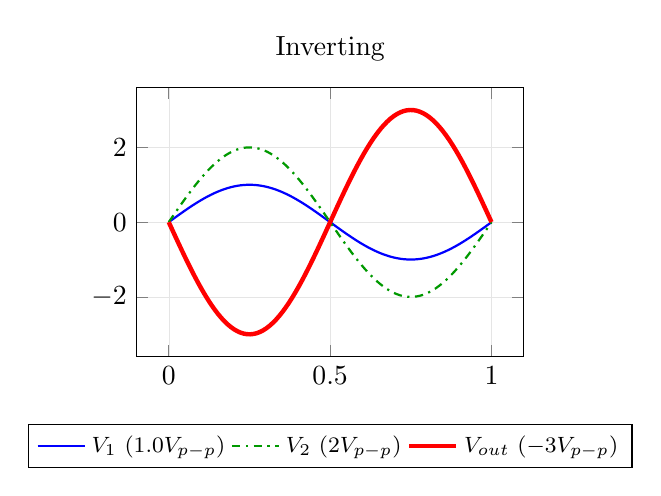
\begin{tikzpicture}
			\begin{axis}[title={Inverting}] % Automatically inherits all settings above!
			% Input V1
				\addplot[thick, blue, domain=0:1, samples=100] {1.0*sin(deg(2*pi*x))};
				\addlegendentry{$V_1\ (1.0\text{ V}_{p-p})$}
				
			%				% Input V2
				\addplot[thick, green!60!black, dashdotted, domain=0:1, samples=100] {2*sin(deg(2*pi*x))};
				\addlegendentry{$V_2\ (2\text{ V}_{p-p})$}
			%				
			% Summed Output Vout = -(V1 + V2)
				\addplot[ultra thick, red, domain=0:1, samples=100] {-3*sin(deg(2*pi*x))};
				\addlegendentry{$V_{out}\ (-3\text{ V}_{p-p})$}
			\end{axis}
%			\begin{axis}[
%				axis lines=middle,
%				xlabel={$t\text{ (ms)}$},
%				ylabel={Voltage (V)},
%				xmin=0, xmax=1,
%				ymin=-3.5, ymax=3.5,
%				grid=both,
%				grid style={line width=.1pt, draw=gray!20},
%				major grid style={line width=.2pt, draw=gray!40},
%				width=5cm, height=5cm,
%				title={\textbf{Inverting Adder ($V_1 = 1.0\text{ V}$, $V_2 = 2\text{ V}$)}},
%				legend pos=outer north east
%				]
				% Input V1
%				\addplot[thick, blue, domain=0:1, samples=100] {1.0*sin(deg(2*pi*x))};
%				\addlegendentry{$V_1\ (1.0\text{ V}_{p-p})$}
%				
%				% Input V2
%				\addplot[thick, green!60!black, dashdotted, domain=0:1, samples=100] {2*sin(deg(2*pi*x))};
%				\addlegendentry{$V_2\ (2\text{ V}_{p-p})$}
%				
%				% Summed Output Vout = -(V1 + V2)
%				\addplot[ultra thick, red, domain=0:1, samples=100] {-3*sin(deg(2*pi*x))};
%				\addlegendentry{$V_{out}\ (-3\text{ V}_{p-p})$}
%			\end{axis}
		\end{tikzpicture}
		\caption{Inverting Summing Amplifier}
		\label{fig:waveforms_adder}
	\end{subfigure}
	\hfill
	\begin{subfigure}[b]{0.42\textwidth}
		\centering
		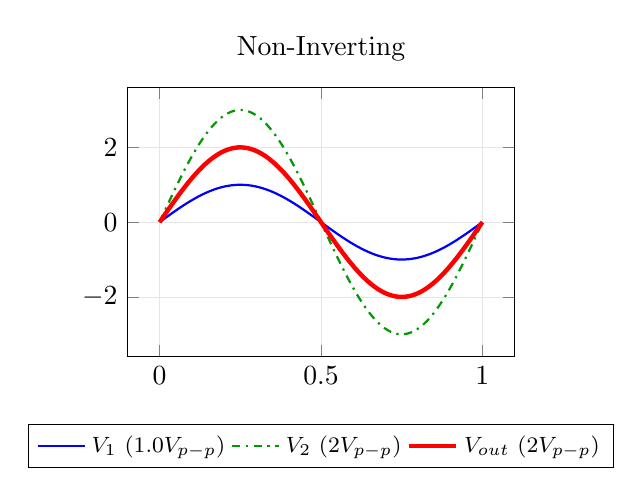
\begin{tikzpicture}
			\begin{axis}[title={Non-Inverting}] % Inherits settings here too!
					% Input V1
				\addplot[thick, blue, domain=0:1, samples=100] {1.0*sin(deg(2*pi*x))};
				\addlegendentry{$V_1\ (1.0\text{ V}_{p-p})$}
				
				% Input V2
				\addplot[thick, green!60!black, dashdotted, domain=0:1, samples=100] {3*sin(deg(2*pi*x))};
				\addlegendentry{$V_2\ (2\text{ V}_{p-p})$}
				
				% Subtracted Output Vout = (V2 - V2)
				\addplot[ultra thick, red, domain=0:1, samples=100] {2*sin(deg(2*pi*x))};
				\addlegendentry{$V_{out}\ (2\text{ V}_{p-p})$}
			\end{axis}
			
%			\begin{axis}[
%				axis lines=middle,
%				xlabel={$t\text{ (ms)}$},
%				ylabel={Voltage (V)},
%				xmin=0, xmax=1,
%				ymin=-3.5, ymax=3.5,
%				grid=both,
%				grid style={line width=.1pt, draw=gray!20},
%				major grid style={line width=.2pt, draw=gray!40},
%				width=5cm, height=5cm,
%				title={\textbf{Subtractor ($V_1 = 1.0\text{ V}$, $V_2 = 1.5\text{ V}$)}},
%				legend pos=outer north east
%				]
%				% Input V1
%				\addplot[thick, blue, domain=0:1, samples=100] {1.0*sin(deg(2*pi*x))};
%				\addlegendentry{$V_1\ (1.0\text{ V}_{p-p})$}
%				
%				% Input V2
%				\addplot[thick, green!60!black, dashdotted, domain=0:1, samples=100] {3*sin(deg(2*pi*x))};
%				\addlegendentry{$V_2\ (2\text{ V}_{p-p})$}
%				
%				% Subtracted Output Vout = (V2 - V2)
%				\addplot[ultra thick, red, domain=0:1, samples=100] {2*sin(deg(2*pi*x))};
%				\addlegendentry{$V_{out}\ (2\text{ V}_{p-p})$}
%			\end{axis}
		\end{tikzpicture}
		\caption{Difference Amplifier}
		\label{fig:waveforms_sub}
	\end{subfigure}
	\caption{Time-Domain Waveforms for Adder and Subtractor}
	\label{fig:waveforms_adder_sub}
\end{figure}

\section{Observation Tables}

\subsection{Adder Circuit DC Measurements}
Record the DC summation observations in Table \ref{tab:dc_adder}.

\begin{table}[h!]
	\centering
	\begin{tabular}{@{}cccc@{}}
		\toprule
		$v_1$ (V) & $v_2$ (V) & $v_3$ (V) & $v_{out}$ (V) \\
		\midrule
		&  &  &  \\
		&  &  &  \\
		&  &  &  \\
		&  &  &  \\
		\bottomrule
	\end{tabular}
	\caption{Summing amplifier: DC observation table (measured vs. Equation~\eqref{eq:adder_gain}).}
	\label{tab:dc_adder}
\end{table}


\subsection{Subtractor Circuit DC Measurements}
Record the DC difference observations in Table \ref{tab:dc_subtractor}.
\begin{table}[h!]
	\centering
	\begin{tabular}{@{}ccccc@{}}
		\toprule
		$v_1$ (V) & $v_2$ (V) & $v_{out}$ (theory) & $v_{out}$ (measured) & \% Error \\
		\midrule
		&  &  &  &  \\
		&  &  &  &  \\
		&  &  &  &  \\
		&  &  &  &  \\
		\bottomrule
	\end{tabular}
	\caption{Difference amplifier: DC observation table (including the equal-input common-mode test).}
	\label{tab:dc_subtractor}
\end{table}

\section{Result}
The performance of Op-Amp Adder and Subtractor circuits using IC 741 was successfully evaluated:
\begin{itemize}
	\item The inverting summing amplifier was verified for DC and AC inputs, confirming that $V_{out} = -(V_1 + V_2)$.
	\item The difference amplifier was verified, confirming $V_{out} = V_2 - V_1$.
\end{itemize}

\section{Questions}
\begin{enumerate}
	\item How can an inverting summing amplifier be modified to compute the mathematical average of three input signals ($V_{out} = -\frac{V_1 + V_2 + V_3}{3}$)?
	\item What happens to the common-mode rejection capability of a subtractor circuit if one of the resistors has a $5\%$ tolerance mismatch?
	\item How would you modify the summing amplifier circuit to perform \emph{subtraction} of two signals using only inverting-adder and inverting-amplifier (unity gain) stages, without using the single-op-amp difference amplifier of Figure~\ref{fig:subtractor_circuit}?
%	\item Why is the matched-ratio condition of Equation~\eqref{eq:cmrr_condition} important for common-mode rejection in the difference amplifier? What happens to the CMRR if $R_3/R_2 \neq R_f/R_1$?
	\item Define Common-Mode Rejection Ratio (CMRR) and explain why a high CMRR is desirable in instrumentation applications.
	\item What is a key limitation of the single-op-amp difference amplifier of Figure~\ref{fig:subtractor} regarding input impedance, particularly when $R_1$ is small? How does an instrumentation amplifier (using three op-amps) overcome this limitation?
	\item If all three inputs of the summing amplifier in Figure~\ref{fig:adder} are driven with the same DC voltage $V$, and $R_1=R_2=R_3=R_f$, what is $v_{out}$? Verify this against your observation table.
	\item Explain, with an example, one practical application each of a summing amplifier and a difference amplifier in analogue signal processing systems.
	\item If $V_1 = \SI{5}{\volt}$ and $V_2 = \SI{10}{\volt}$ are applied to an adder configured with unity gain powered at $\pm 15\text{ V}$, will the output be $-15\text{ V}$? Explain why or why not.
	\item Describe how a non-inverting summing amplifier can be designed using a single op-amp.
\end{enumerate}
